\subsection{Metric}
%\begin{table}
%\begin{tabular}{|c|p{6.5cm}|}
%\hline
%Score & Description \\
%\hline
%0 & Re-write the whole method \\
%\hline
%1 & The translated method seems to be incorrect. You are hesitate to fix and use it. \\
%\hline
%2 &  You see something wrong, but may fix and use it. \\
%\hline
%3 & The translated method seems to be correct. You are willing to fix and use it. \\
%\hline
%4 & The methods are identical. You do not need to change anything and can use it as is. \\
%\hline
%\end{tabular}
%\caption{Manual Semantic Score Criteria}
%\label{table:criteria}
%\end{table}

\begin{table}
\begin{tabular}{|c|p{6.5cm}|}
\hline
Score & Description \\
\hline
0 & The translated method is totally useless. One needs to rewrite the whole method. \\
\hline
1 & The translated method seems to be incorrect. Even though some parts are reusable, it is not worth to fix and use the method. \\
\hline
2 &  It cannot be decided if the translated method is useful or not. \\
\hline
3 & The translated method seems to be correct. Even though it needs some adjustments, it is worth to use the method. \\
\hline
4 & The methods are identical in term of functionality. There is no change needed and it can be use as-is. \\
\hline
\end{tabular}
\caption{Manual Semantic Score Criteria}
\label{table:criteria}
\end{table}

%\textbf{Semantic Score.}
%To answer the question whether BLEU score reflect semantic of source code, 
%Before one can answer the question whether BLEU score reflects semantic accuracy of translated source code or not, it is necessary to define what is the semantic accuracy. Given a pair of methods: one generated by SMT-based migration system and another one is the reference code written by real developers, the semantic accuracy is expressed by the similarity in term of functionality between the two. If the two methods perform the same functionality, they are semantically similar.

Remind that our goal of the experiment is to (in)validate whether BLEU
reflects the semantic accuracy of the migrated code from the tools
with respect to the manual-migrated code in the collected ground
truth. 
%
Semantic accuracy between pairs of methods (one is the result from a
SMT-based migration tool and another is the reference code from the
ground truth) is the similarity between them in term of execution and
functionality. If two methods perform similar operations on a given
input, they are semantically similar, even interchangeable. A pair of
methods can have the same functionality despite of their difference in
term of program elements.
%
For example, a method using a \code{for} loop and a method using a
\code{while} loop, they still can perform the same functionality even
though their lexical representations are much different. There exist
many studies aiming to measure the functionality similarity of source
code, which utilize the similarities of structures and
dependencies~\cite{clone-tse07,roy09,ducasse99,baker97,ccfinder,cpminer,baxter98,deckard,deckard2,horwitz01}.
%
However, they are not reliable as their results sometimes contradict
with human judgments on semantic accuracy~\cite{fse14-higo}. More
importantly, those structure-based metrics {\em do not reflect human
  efforts} in fixing the incorrect migrated code into the correct one.
%
Human judgment for our study would be the most reliable metric to
measure semantic accuracy. A developer who examines a pair of methods
can tell whether the code perform the same functionality as well as
explain the efforts needed for the correction. Therefore, we conducted
a study that used a human subject to manually evaluate the migrated
code from the SMT-based migration tools.
%2 goals

%Our study was conducted as follows:

\emph{1. Sample Size}. Because our dataset contains a large number of pairs of methods, it would take a lot of efforts to manually evaluate all of them. According to \cite{website}, from a population of 34,209, a sample size of 375 is reasonable as it has confidence level of $95\%$ and margin of error $5\%$. Then, we randomly sampled 375 pairs of methods from the dataset to evaluate. 

\emph{2. Setting}. The human subject of our study is one of the authors who is fluent in both Java and C\#. He was then given a pair of methods in C\#: one was the translated method generated by SMT and another one was the reference code originally written by real developers (for example: a pair of method in figure xxx). Each method was labeled clearly as reference or machine-generated code. He was also given the original Java method to understand the requirements of the migration task for this method. Moreover, he was provided with the github links to the contended projects (both Java and C\# versions) where those methods came from so that he could refer back to the context of the methods.

\emph{3. Scoring.} Finally, the human subject was told to give a score
for each of 375 pairs of methods. We set two goals for the human
subject in evaluting the results. The first goal is the correctness of
the resulting code with respect to the manual-migrated code in the
ground truth. The second one is based on the efforts needed to correct
the translated code to achieve the same functionaity as of the
reference code in the ground truth.
%
%The scoring was based on the human efforts needed to fix the
%translated method to achieve the same functionality as of the
%reference one.
%
Score ranges from 0 to 4 as follows: A score of 0 means the translated
method is totally useless, and it is better to re-write the whole
method rather than use it. A score of 1 means the translated method
seems incorrect, and even though some parts of it are reusable, the
human subject do not want to fix and use it. A score of 2 means the
human subject cannot decide whether to use the translated method or
not. A score of 3 means the translated method seems correct, but it
still needs some minor adjustments. A score of 4 means the pairs of
methods are identical in term of functionality, and the translated
method can be used as-is. In short, the scoring guidelines are listed
on Table \ref{table:criteria}. Before actually giving the scores, the
human subject could study our preselected examples with according
scores and explanation. The examples are presented on Figure
\ref{fig:scoreEG}. Specifically, code from line 11 to line 20
represents a score of 4. Noted that even though it is different from
the reference code in term of tokens (use a normal for loop instead of
a for each), it still performs the same functionality. A translated
method of score 3 (lines 21 to line 30) seems to have similar
functionality as the reference code, but it still needs some minor
adjustment (line 23 wrong function call: indexOf instead of IndexOf,
wrong parameter). Lines 31 to 40 demonstrates a translated method
which has score of 3. It cannot be decided if the method should be
used or not. It has some good program elements that similar to the
reference code, but at the same time, has some critical errors that
would be hard to fix. A translated method of score 1 (lines 41 to 50)
has only one line of code reusable (line 43). So it is not worth it to
fix and use the method. Lines 51 to 60 represents a translated code of
score 0 which means the whole method is totally useless. It is better
to rewrite the whole method.
%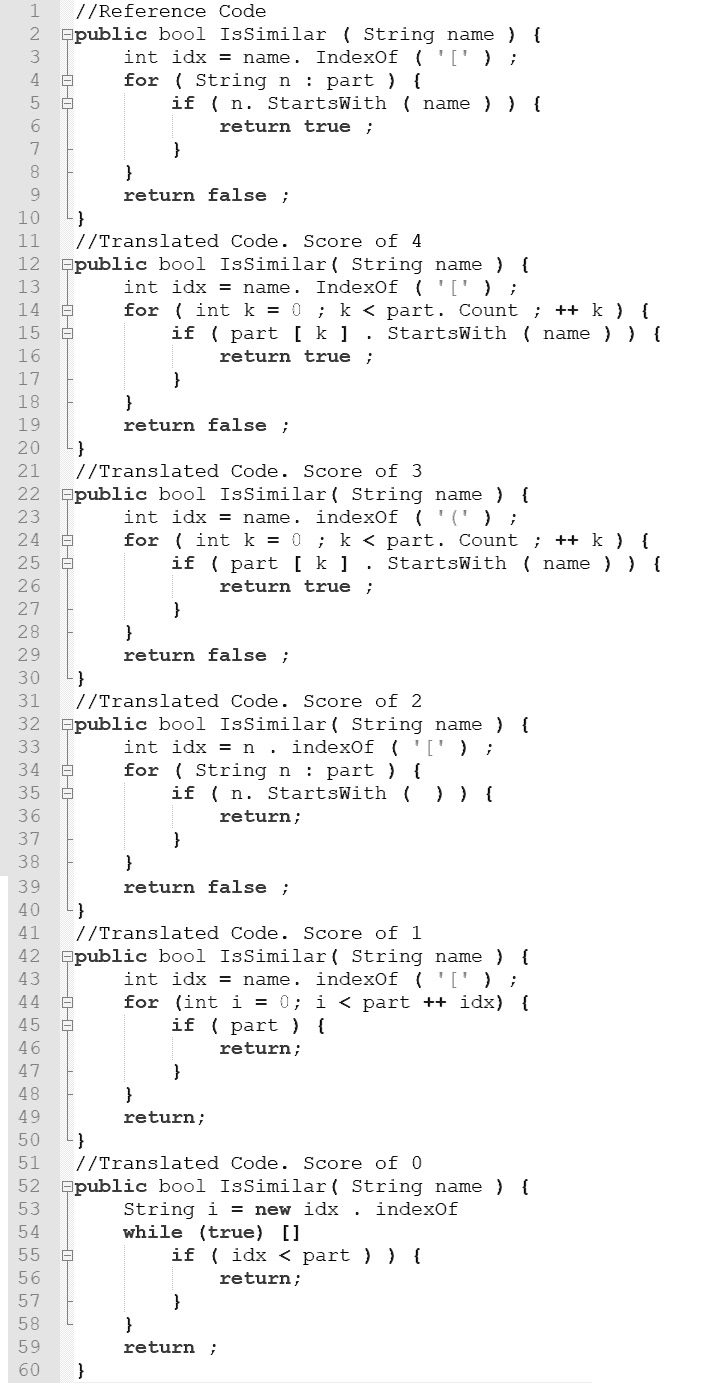
\includegraphics{scoreExamples}

We conducted the same human study for the results of both lpSMT and mppSMT models. As a result, we have scores for 375 pairs of methods for each model. From now on, we regard those scores as \textbf{Semantic Score}.

\begin{figure}
\caption{Scoring Examples}
\centering
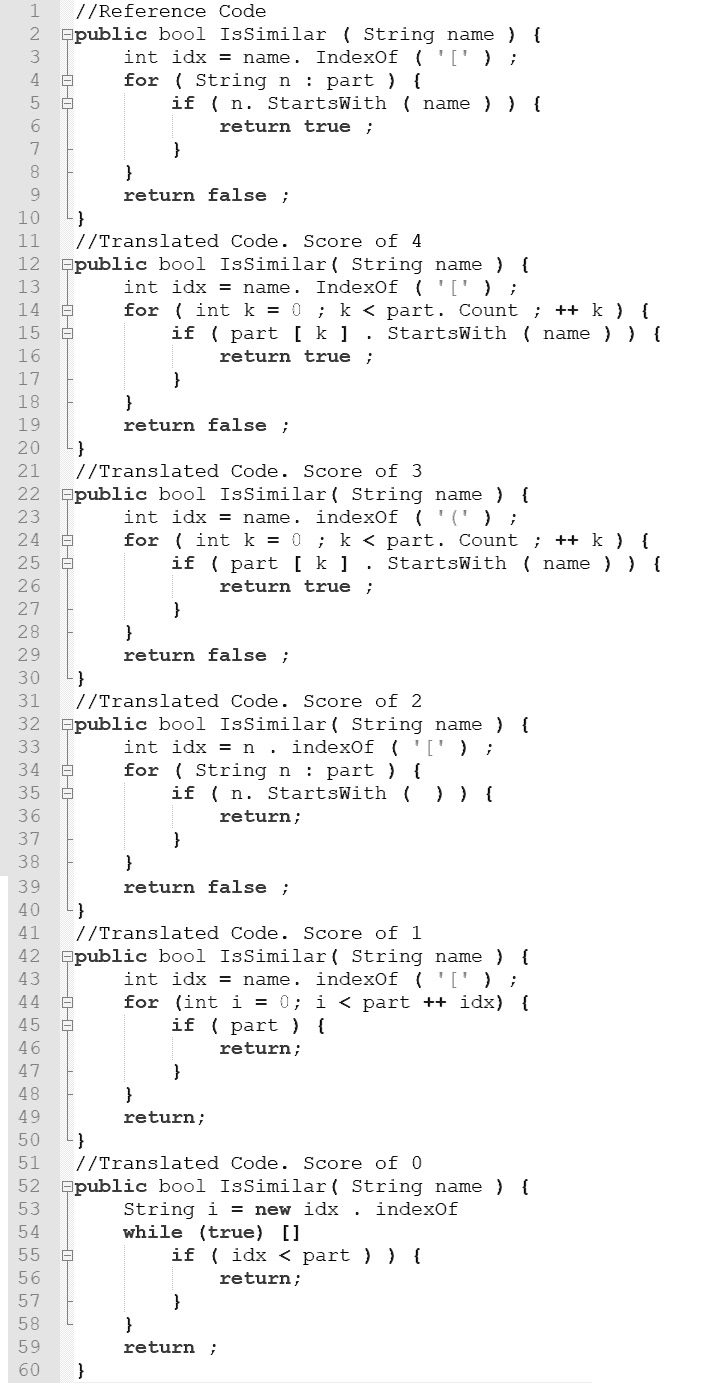
\includegraphics{scoreExamples}
\label{fig:scoreEG}
\end{figure}


%Our hypothesis states that \emph{\textit{BLEU score does not measure well the similarity in term of semantics between the reference and migrated source code}}. Therefore, given a pair of methods (reference one and machine translated one), we need a metric that can measure the similarity in term of semantics between them. As we know of, there is no automated metrics to do that task. To determine semantic similarity score, we used a human subject to manually evaluate pairs of methods to see how close they are in term of semantic/functionality. Specifically, scoring is done based on the human effort to fix the translated method to achieve the same functionality as of the reference one. The detailed scoring guidelines are presented in Table\ref{table:criteria}. The human subject is a senior developer who is fluent in both Java and C\#. He was given a pair of methods in C\# (machine generated one and reference one), the original method in Java, and the context project from which the methods come from. Then, he was told to evaluate pairs of methods in C\#, and give score as our guideline above and table \ref{table:criteria}. He could also refer back to the original Java method and project for a better understanding of the context. Below are examples for each score from -2 to 2:\\
%To determine semantic similarity score between pair of methods, we manually scored each pair from 0 to 6 based on the human effort to fix a translated method to a referenced one. Specifically, we list the criteria to score in Table  with a score of 0 means the pair of methods are totally different, and a score of 6 means they are totally the same. Scoring also follows the following principles: 1. An effort to fix a syntactical error (misplacing a semi-colon, parenthesis...) has less weight than an effort to fix a semantical error (wrong branch, wrong function call...). 2. A fix that requires adding sources code has more weight than one that requires removing/replacing. 3. A fix for user-defined program elements (identifier, simple name, method name) is more 'pricey' than a fix for keyword (this, if, for...). Example (of scores 1,3,5). 

%Since our dataset contains a large number of pairs of methods, it would take a lot of efforts to manually evaluate all of them. Hence, we took a sample from our population of total 34,209 pairs. According to \cite{website}, our sample size is 375 with confidence level of $95\%$ and margin of error $5\%$. After we conducted the human experiment with 375 pairs of methods, we normalized the result on 0-1 range with 0 is respected to -2 and 1 is respected to 2. 
